%% Standalone figure: compile this file once (pdflatex sphere.tex) to produce sphere.pdf,
%% which main.tex includes with \includegraphics. Recompile only after editing the figure.
\documentclass[11pt,tikz,border=2pt]{standalone}
\usepackage{amsmath,amssymb}       % \text, \vec, math symbols
\usetikzlibrary{arrows.meta}       % Stealth arrow tips
\begin{document}
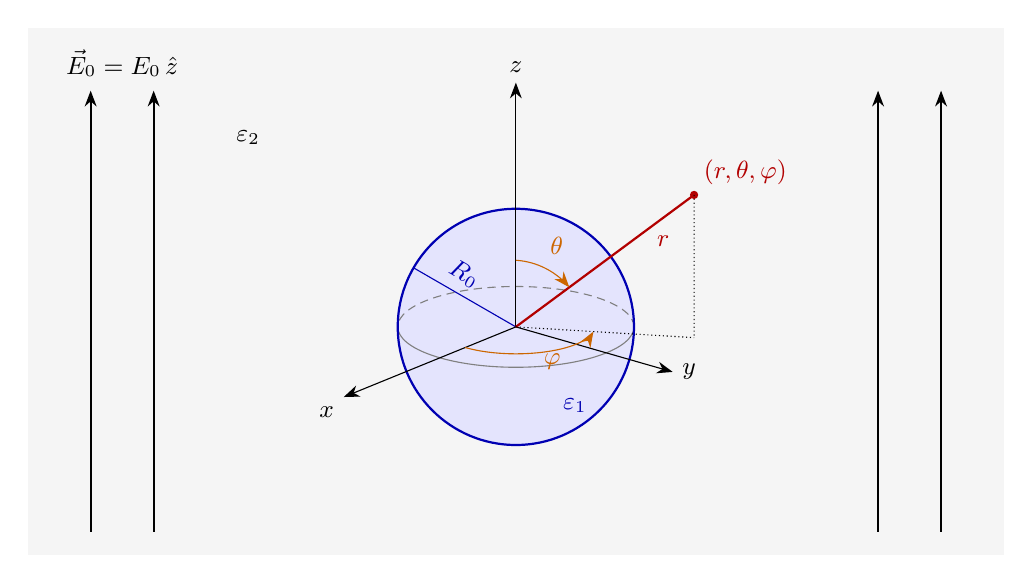
\begin{tikzpicture}[
  font=\small,
  >={Stealth[length=2mm]},
  % orthographic view: azimuth 40 deg, elevation 20 deg
  x={(-0.643cm,-0.262cm)}, y={(0.766cm,-0.220cm)}, z={(0cm,0.940cm)},
]
  \def\Rs{1.5}                       % sphere radius R_0 (cm)
  \pgfmathsetmacro{\Re}{\Rs*0.342} % equator semi-minor axis = R_0 sin(elevation)
  \def\rr{3.0}  \def\th{50}  \def\ph{120}   % field point (r, theta, varphi)

  % ---------- medium 2 and the uniform external field ----------
  \fill[gray!8] (-6.2cm,-2.9cm) rectangle (6.2cm,3.8cm);
  \foreach \X in {-5.4,-4.6,4.6,5.4}{
    \draw[->, thick] (\X cm,-2.6cm) -- (\X cm,3.0cm);
  }
  \node[anchor=south] at (-5.0cm,3.05cm) {$\vec E_0 = E_0\,\hat z$};
  \node at (-3.4cm,2.4cm) {$\varepsilon_2$};

  % ---------- sphere (medium 1) ----------
  \fill[blue!12, opacity=0.8] (0cm,0cm) circle (\Rs cm);
  \draw[densely dashed, gray] (\Rs cm,0cm) arc (0:180:\Rs cm and \Re cm);
  \draw[gray] (-\Rs cm,0cm) arc (180:360:\Rs cm and \Re cm);
  \draw[thick, blue!70!black] (0cm,0cm) circle (\Rs cm);
  \node[blue!70!black] at (0.75cm,-1.0cm) {$\varepsilon_1$};
  \draw[blue!70!black] (0cm,0cm) -- (150:\Rs cm) node[pos=0.6, above, sloped] {$R_0$};

  % ---------- Cartesian axes ----------
  \draw[->] (0,0,0) -- (3.4,0,0) node[anchor=north east] {$x$};
  \draw[->] (0,0,0) -- (0,2.6,0) node[anchor=west] {$y$};
  \draw[->] (0,0,0) -- (0,0,3.3) node[anchor=south] {$z$};

  % ---------- field point P and its spherical coordinates ----------
  \coordinate (P)  at ({\rr*sin(\th)*cos(\ph)},{\rr*sin(\th)*sin(\ph)},{\rr*cos(\th)});
  \coordinate (Pp) at ({\rr*sin(\th)*cos(\ph)},{\rr*sin(\th)*sin(\ph)},0);
  \draw[thick, red!70!black] (0,0,0) -- (P) node[pos=0.75, below right=-1pt] {$r$};
  \fill[red!70!black] (P) circle (1.5pt) node[anchor=south west] {$(r,\theta,\varphi)$};
  \draw[densely dotted] (P) -- (Pp) (0,0,0) -- (Pp);
  % polar angle theta, measured from the z axis
  \draw[->, orange!80!black, domain=0:\th, samples=30]
    plot ({0.9*sin(\x)*cos(\ph)},{0.9*sin(\x)*sin(\ph)},{0.9*cos(\x)});
  \node[orange!80!black] at ({1.25*sin(\th/2)*cos(\ph)},{1.25*sin(\th/2)*sin(\ph)},{1.25*cos(\th/2)}) {$\theta$};
  % azimuthal angle varphi, measured from the x axis in the xy plane
  \draw[->, orange!80!black, domain=0:\ph, samples=40]
    plot ({1.0*cos(\x)},{1.0*sin(\x)},0);
  \node[orange!80!black] at ({1.35*cos(\ph/2)},{1.35*sin(\ph/2)},0) {$\varphi$};
\end{tikzpicture}
\end{document}
